\documentclass[tikz]{standalone}
\usepackage{pgfplots}
\pgfplotsset{compat=1.15}
\usepackage{mathrsfs}
\usetikzlibrary{arrows,calc}
\usepackage{tkz-euclide}

\pagestyle{empty}

\definecolor{AngleClr}{rgb}{0,0.39215686274509803,0}
\definecolor{ShapeClr}{rgb}{0.6,0.2,0}

\begin{document}

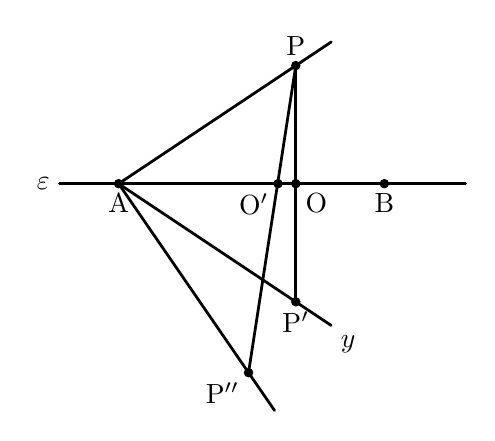
\begin{tikzpicture}[scale=.75]
\tkzSetUpLine[line width=1pt,color=black]
\tkzSetUpPoint[fill=black]

\tkzDefPoints{0/0/A,3/2/P,3/-2/PP,3/0/O,2.7/0/OO,2.2/-3.2/PPP,4.5/0/B,-1/0/E1}


\tkzDefPointOnLine[pos=1.2](A,PP)\tkzGetPoint{y}

\tkzDrawSegments[line width=1pt,color=black,add=0 and 0.2](A,P A,PP A,PPP)
\tkzDrawSegments[line width=1pt,color=black](P,PP P,PPP)
\tkzDrawSegments[line width=1pt,color=black,add=0. and 0.25](E1,B)

% \tkzMarkRightAngle[line width=1pt, size=.3,color=AngleClr,fill=AngleClr,fill opacity=0.1](y',O,x')

\tkzDrawPoints[size=3](O,OO,P,PP,PPP,A,B)
\tkzLabelPoint[below right](O){$\rm O$}

\tkzLabelPoint[below left](OO){${\rm O}'$}
\tkzLabelPoint[below left](PPP){${\rm P}''$}
\tkzLabelPoint[below](PP){${\rm P}'$}
\tkzLabelPoint[above](P){${\rm P}$}

\tkzLabelPoint[left](E1){$\varepsilon$}
\tkzLabelPoint[below right](y){$y$}

\tkzLabelPoint[below](A){${\rm A}$}
\tkzLabelPoint[below](B){${\rm B}$}

\end{tikzpicture}

\end{document}
